\thispagestyle{empty} %Oculta o numero da primeira pagina do capitulo
\vspace{3ex}


\chapter{Estudo de viabilidade do método KPLS na predição de vida em fadiga.}
\label{finalsec}

\section{Introdução}
% O método KPLS (Kriging e médios quadrados parciais), quando usado na predição de séries temporais de tensão, pode resultar em boas aproximações a baixos custos computacionais.

Neste segmento procura-se estudar os impactos da utilização do método KPLS (\emph{Kriging model and partial least squares}) na predição de séries temporais de tensão para aplicação no estudo da vida em fadiga dos elementos estruturais. No caso deste estudo, a análise é feita a partir das tensões externas de Von Mises desenvolvidas a partir do software Anflex do CENPES/PETROBRAS. O caso analisado consiste em um longo \emph{riser} com flutuadores (Fig. \ref{figure.1}) que tornam flutuante parte da estrutura submersa (configuração \emph{lazy-wave}). 

\begin{figure}[!h]
    \centering
    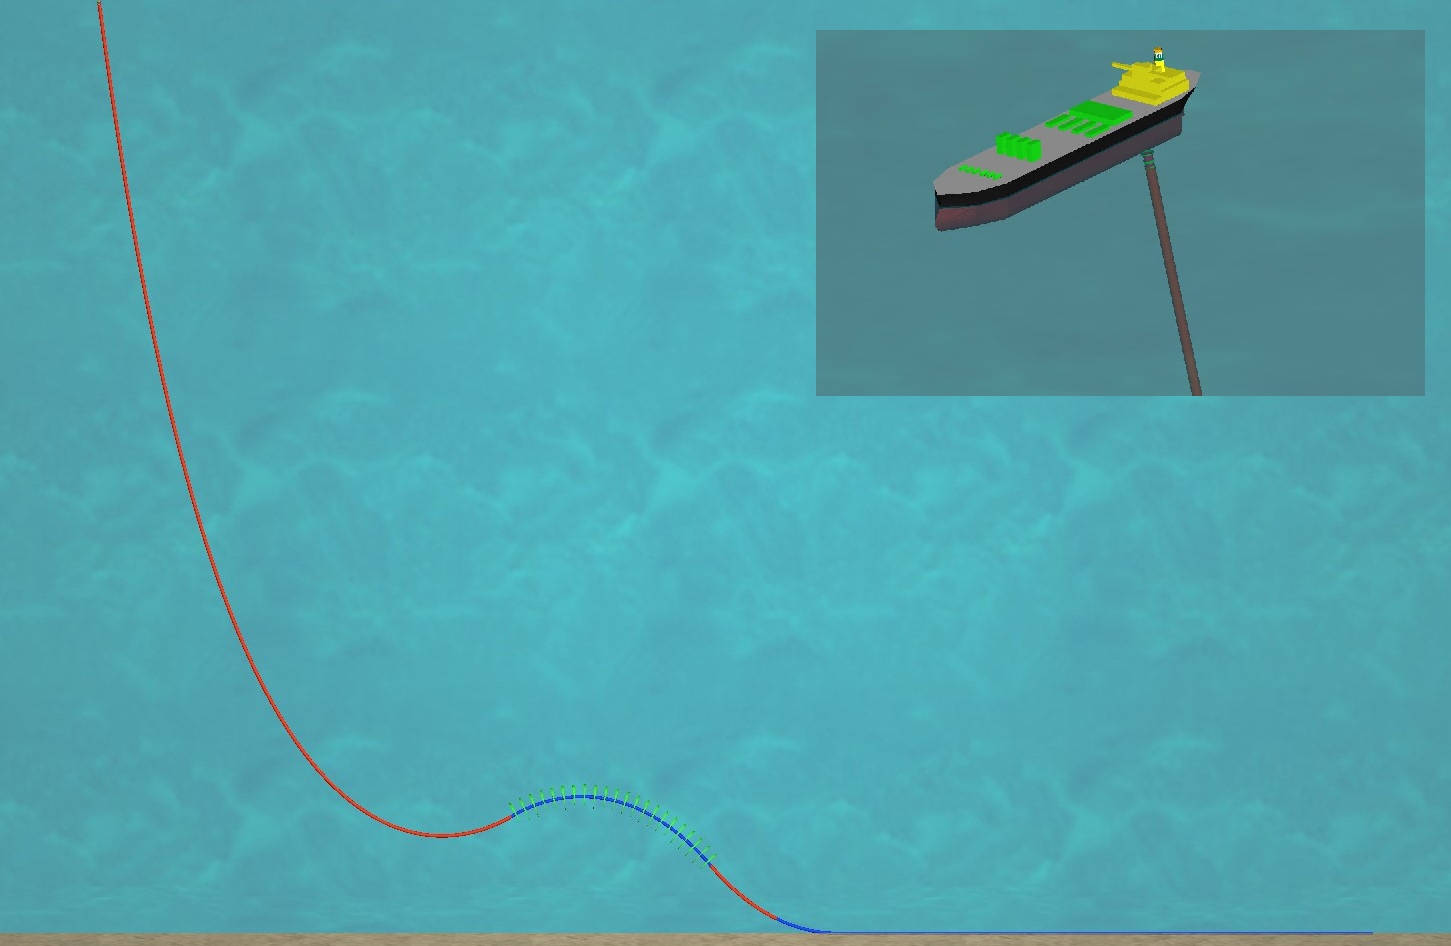
\includegraphics[width=0.5\linewidth , trim = {40mm 0mm 30mm 5mm} , clip]{felipe/fig_felipe/caso_estudado.jpg}
    \caption{Configuração \emph{lazy-wave}, onde o estudo foi desenvolvido.}
    \label{figure.1}
\end{figure}

O segmento flutuante (denominado região de SAG/HOG) tem o objetivo de atenuar os carregamentos advindos dos deslocamentos da estrutura flutuante ào segmento do riser em contato com o leito marinho. Seus efeitos podem ser observados no andamento deste estudo ao causar notável influencia na vida em fadiga dos elementos próximos. 

A biblioteca SMT foi utilizada para aplicação do método KPLS. Este pacote possui muitas ferramentas de metamodelo também aplicadas neste projeto \textbf{(BOUHLELet al., 2019)}.

Dessa forma, tem-se o intúito de se aplicar o método \emph{RainFlow} e o método de Goodman modificado para determinação da vida em fadiga a partir das séries de tensões externas de Von Mises advindas das simulações feitas no Anflex. O método KPLS é utilizado para predição parcial destas séries e então se calcula a vida em fadiga destas séries parcialmente ajustadas. Comparando-se os resultados observou-se boa conformidade, o que levanta boas oportunidades de otimização ao tornar facultativo o desenvolvimento de uma simulação completa para este tipo de análise. 

% Como mencionado, o pacote SMT foi utilizado para determinar os resultados deste relatório parcial. Os seguintes metamodelos est ̃ao disponíveis nesta biblioteca Python (BOUHLELet al., 2019)

% desenvolver um algorítmo com o qual se possa analisar a vida em fadiga a partir das séries temporais de tensão advindas do software Anflex. Além disso este programa deve ser capaz de fazer a predição de séries temporais de tensão a partir do médo KPLS. Dessa forma, com a rotina se comparará os valores de vida em fadiga a partir dos dados de tensão completamente simulados pelo Anflex e a partir dos dados parcialmente ajustados com o método KPLS.

\section{Metodologia}

\subsection{Método RainFlow}

\subsection{Método de Goodman modificado}

\subsection{Método KPLS de predição de séries temporais}

\subsection{Análise introdutória da vida em fadiga}



